% ============================================================
%  Piezoelectric Actuator Preload Diagrams
%  Figure 1: Mass Preload
%  Figure 2: Spring Preload
%
%  Compile with: pdflatex piezo_preload_diagrams.tex
%  Requires: tikz, decorations.pathmorphing library
% ============================================================

\documentclass[border=6pt]{standalone}
\usepackage{tikz}
\usetikzlibrary{
	patterns,
	arrows.meta,
	decorations.pathmorphing,
	decorations.pathreplacing,
	calc
}
\usepackage{amsmath}

% ---- Colour palette ----------------------------------------
\colorlet{PGreen}{green!55!black}   % piezo A (green)
\colorlet{PRed}{red!65!black}       % piezo B (red)
\colorlet{LBlue}{cyan!55!blue}      % load line / operating region

% ---- Reusable: striped piezo block -------------------------
%  #1 x-left  #2 y-bottom  #3 x-right  #4 y-top  #5 color
\newcommand{\piezoblock}[5]{%
	\begin{scope}
		\clip (#1,#2) rectangle (#3,#4);
		\foreach \ii in {0,...,22}{%
			\fill[#5!72] (#1,{#2+\ii*0.205}) rectangle (#3,{#2+\ii*0.205+0.135});
		}
	\end{scope}
	\draw[thick] (#1,#2) rectangle (#3,#4);
}

% ---- Reusable: floor-ground symbol -------------------------
%  #1 x-centre  #2 y-line  #3 half-width
\newcommand{\gnd}[3]{%
	\draw[thick] ({#1-#3},#2) -- ({#1+#3},#2);
	\fill[pattern=north east lines, pattern color=black!55]
	({#1-#3},{#2-0.28}) rectangle ({#1+#3},#2);
}

% ---- Reusable: ceiling-mount symbol (hatching above line) --
%  #1 x-left  #2 x-right  #3 y-line
\newcommand{\ceiling}[3]{%
	\draw[thick] (#1,#3) -- (#2,#3);
	\fill[pattern=north east lines, pattern color=black!55]
	(#1,#3) rectangle (#2,{#3+0.28});
}

% ---- Reusable: vertical coil spring ------------------------
%  #1 x  #2 y-start  #3 x (same)  #4 y-end
\newcommand{\springV}[4]{%
	\draw[thick,
	decoration={coil, aspect=0.38, segment length=3.5pt, amplitude=4.5pt},
	decorate] (#1,#2) -- (#3,#4);
}

% ---- Shared hysteresis loop A (green, wider band) ----------
%  #1=x-graph-origin  #2=y-graph-origin
\newcommand{\loopA}[2]{%
	\fill[PGreen!28]
	({#1+0.15},{#2+0.10})
	.. controls ({#1+1.25},{#2+0.98}) and ({#1+2.35},{#2+2.05}) ..
	({#1+3.15},{#2+3.13})
	.. controls ({#1+2.72},{#2+2.90}) and ({#1+1.72},{#2+1.82}) ..
	({#1+0.00},{#2+0.06}) -- cycle;
	\draw[PGreen!85!black, line width=1.4pt]
	({#1+0.15},{#2+0.10})
	.. controls ({#1+1.25},{#2+0.98}) and ({#1+2.35},{#2+2.05}) ..
	({#1+3.15},{#2+3.13});
	\draw[PGreen!85!black, line width=1.4pt]
	({#1+0.00},{#2+0.06})
	.. controls ({#1+1.72},{#2+1.82}) and ({#1+2.72},{#2+2.90}) ..
	({#1+3.15},{#2+3.13});
	\node[PGreen!78!black, font=\bfseries] at ({#1+1.35},{#2+2.78}) {A};
}

% ---- Shared hysteresis loop B (red, narrower band) ---------
%  #1=x-graph-origin  #2=y-graph-origin
\newcommand{\loopB}[2]{%
	\fill[PRed!28]
	({#1+0.08},{#2+0.04})
	.. controls ({#1+1.10},{#2+0.55}) and ({#1+2.35},{#2+1.65}) ..
	({#1+3.20},{#2+2.30})
	.. controls ({#1+2.10},{#2+1.98}) and ({#1+0.72},{#2+0.82}) ..
	({#1+0.08},{#2+0.04}) -- cycle;
	\draw[PRed!85!black, line width=1.4pt]
	({#1+0.08},{#2+0.04})
	.. controls ({#1+1.10},{#2+0.55}) and ({#1+2.35},{#2+1.65}) ..
	({#1+3.20},{#2+2.30});
	\draw[PRed!85!black, line width=1.4pt]
	({#1+0.08},{#2+0.04})
	.. controls ({#1+0.72},{#2+0.82}) and ({#1+2.10},{#2+1.98}) ..
	({#1+3.20},{#2+2.30});
	\node[PRed!85!black, font=\bfseries] at ({#1+2.45},{#2+1.60}) {B};
}

\newcommand{\loopC}[2]{%
	\fill[PRed!28]
	({#1+0.15},{#2+0.10})
	.. controls ({#1+1.25},{#2+0.98}) and ({#1+2.35},{#2+2.05}) ..
	({#1+3.15},{#2+3.13})
	.. controls ({#1+2.72},{#2+2.90}) and ({#1+1.72},{#2+1.82}) ..
	({#1+0.00},{#2+0.06}) -- cycle;
	\draw[PRed!85!black, line width=1.4pt]
	({#1+0.15},{#2+0.10})
	.. controls ({#1+1.25},{#2+0.98}) and ({#1+2.35},{#2+2.05}) ..
	({#1+3.15},{#2+3.13});
	\draw[PRed!85!black, line width=1.4pt]
	({#1+0.00},{#2+0.06})
	.. controls ({#1+1.72},{#2+1.82}) and ({#1+2.72},{#2+2.90}) ..
	({#1+3.15},{#2+3.13});
	\node[PRed!78!black, font=\bfseries] at ({#1+1.35},{#2+2.58}) {B};
}

% ============================================================
\begin{document}
	% ============================================================
	
	%% ===========================================================
	%%  FIGURE 1 -- Mass Preload
	%% ===========================================================
	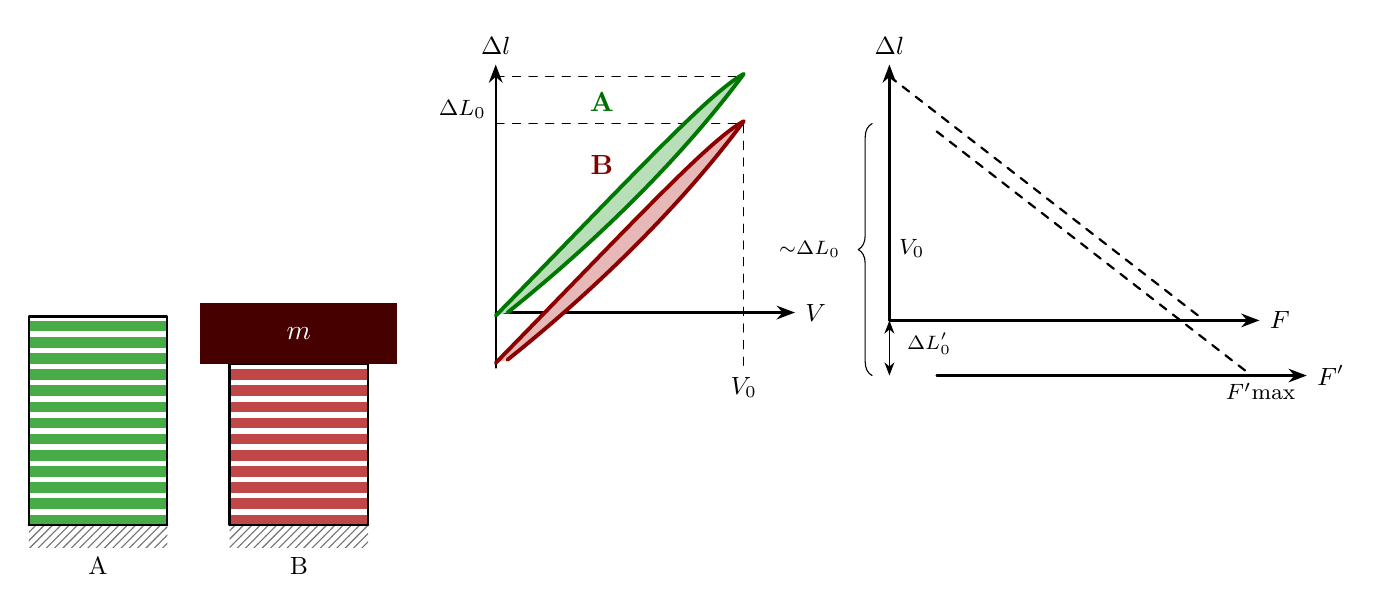
\begin{tikzpicture}[font=\small, >=Stealth, line cap=round, line join=round]
		
		% -- Actuator A (green, floor-mounted) -----------------------
		\gnd{-4.35}{0}{0.88}
		\piezoblock{-5.23}{0}{-3.47}{2.65}{PGreen}
		\node[below=8pt] at (-4.35,0) {A};
		
		% -- Actuator B (red, floor-mounted) + mass block ------------
		\gnd{-1.80}{0}{0.88}
		\piezoblock{-2.68}{0}{-0.92}{2.05}{PRed}
		\fill[PRed!42!black] (-3.05,2.05) rectangle (-0.55,2.82);
		\node[white, font=\bfseries\normalsize] at (-1.80,2.43) {$m$};
		\node[below=8pt] at (-1.80,0) {B};
		
		% -- Center: DeltaL vs V graph --------------------------------
		% Graph origin
		\def\Gox{0.7}
		
		\draw[->,thick] (\Gox,2.7) -- ({(\Gox)+3.8},2.7) node[right] {$V$};
		\draw[->,thick] (\Gox,2) -- (\Gox,5.85)       node[above] {$\Delta l$};
		
		\draw[dashed,thin]
		(\Gox,5.1) -- ({(\Gox)+3.15},5.1) -- ({(\Gox)+3.15},2)
		node[below] {$V_0$};
		\draw[dashed,thin]
		({(\Gox)},5.7) -- ({(\Gox)+3.15},5.7);

		\node[left,font=\footnotesize] at (\Gox,5.28) {$\Delta L_0$};
		
		\loopA{\Gox}{2.6}
		\loopC{\Gox}{2} %need to make this red and labelled B
		
		% -- Right: DeltaL vs F graph (mass preload) -----------------
		% Graph origin
		\def\Fox{5.7}
		
		\draw[->,thick] (\Fox,2.6) -- ({(\Fox)+4.7},2.6) node[right] {$F$};
		\draw[->,thick] (\Fox+.6,1.9) -- ({(\Fox)+.6+4.7},1.9) node[right] {$F'$};
		\draw[->,thick] (\Fox,2.6) -- (\Fox,5.85)       node[above] {$\Delta l$};
		
		% V0 label top-left
		\node[above right, font=\footnotesize] at (\Fox,3.28) {$V_0$};
		
		% Upper dashed stroke line (actuator A at V0)
		\draw[dashed, thick]
		(\Fox,5.7) -- ({(\Fox)+4},2.6);
		
		% Lower dashed stroke line (actuator B at V0)
		\draw[dashed, thick]
		(\Fox+.6,5) -- ({(\Fox)+4.6},1.9);
		\node[right,font=\footnotesize] at ({(\Fox)+4.15},1.7) {$F'\text{max}$};
		
		% DeltaL0' double arrow (between the two y-intercepts)
		\draw[<->,thin]
		({(\Fox)},2.6) -- ({(\Fox)},1.9);
		\node[right,font=\scriptsize] at ({(\Fox)+0.1},2.3) {$\Delta L_0'$};
		
		% ~DeltaL0 brace (from y=0 to y=DeltaL0')
		\draw[decoration={brace, amplitude=5pt}, decorate]
		({(\Fox)-0.22},1.9) -- ({(\Fox)-0.22},5.1);
		\node[left,font=\scriptsize] at ({(\Fox)-0.5},3.5) {${\sim}\Delta L_0$};
		
	\end{tikzpicture}
	
\end{document}